\subsubsection{The Kaus (2010) Brick}
\label{sec:benchmarks-the-kaus_2010-brick}

\textit{This section was contributed by John Naliboff, Marcel Saaro and Cedric Thieulot.}

This setup is based on from Kaus (2010) \cite{kaus10} and the  prm file is in {\tt /benchmarks/viscoelastic\_plastic\_shear\_bands}. The domain is a Cartesian box of size $(L_x \times L_y)=(\SI{40}{km} \times \SI{10}{km})$.
The setup is shown in Fig.~\ref{fig:kaus_brick}. 
The viscous inclusion of size $(\SI{800}{m} \times \SI{400}{m})$ is centered at the bottom of the domain. Its viscosity is $\eta_i=\SI{1e20}{\pascal\second}$.

The brick material is characterised by an (elasto-)visco-plastic
rheology following a Drucker-Prager yield criterion with a cohesion $c=\SI{40}{\mega\pascal}$ and angle of 
friction $\phi=\SI{30}{\degree}$. The elastic shear modulus is set to $G=\SI{50e10}{\pascal}$.

Both materials (brick and inclusion) have a density of $\rho=\SI{2700}{\kg\per\cubic\meter}$. The gravity is pointing downwards with $g=\SI{10}{\meter\per\square\second}$.
The flow is assumed to be isothermal and incompressible.

The boundary conditions are free slip at the bottom and sides and stress free at the top (free surface). The horizontal component of the velocity is prescribed on the sides such that it results in a background strainrate of $\dot{\varepsilon}=\SI{2e-15}{\per\second}$. By reversing the velocity directions on both sides the brick can be put in compression or extension. 

The mesh is composed of $100\times25$ repetitions, i.e. a resolution of $\SI{400}{\m}$ in the absence of further refinement. The model runs for $\SI{20}{\kilo year}$.

\begin{figure}[h]
\centering
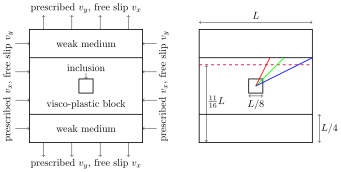
\includegraphics{../../benchmarks/viscoelastic_plastic_shear_bands/kaus_2010/doc/kaus_2010_brick_setup.pdf}
\caption{\it Setup for the Kaus (2010) brick in compression.}
\label{fig:kaus_brick}
\end{figure}

Figure~\ref{fig:kaus_brick_result} shows the effective strain rate field at 3 different times as obtained with the python script included in the corresponding folder. Elastic stresses build up until the yield criterion is reached and plastic deformation is activated, ultimately generating two conjugated shear bands rooted on the inclusion.

\begin{figure}[h]
\centering
\includegraphics[width=12cm]{../../benchmarks/viscoelastic_plastic_shear_bands/kaus_2010/doc/kaus10_vep.pdf}
\caption{\it Time evolution of the shear bands in the extensional case.}
\label{fig:kaus_brick_result}
\end{figure}
